\listfiles
\documentclass{scrartcl}
\usepackage[T1]{fontenc} 
\usepackage{libertine}
\usepackage[scaled=0.88]{beramono}
\usepackage[utf8]{inputenc} 
\usepackage{listings}
%
\lstset{%
    language=[LaTeX]TeX,%
    showstringspaces=false,%
    tabsize=5,%
%    frame={tb},%
%    lineskip=-1pt,%
    extendedchars=true,%
    basicstyle={\footnotesize\ttfamily},%
    numbers=left,%
    stepnumber=1,%
    numberstyle=\tiny,%
%    xleftmargin=2em,%
    breaklines=true}
%
\usepackage[fbox]{hvfloat}
\let\hvVersion\fileversion
\usepackage{graphicx}
\usepackage{url}
\usepackage{tabularx}
\usepackage{lscape}
\usepackage{multicol}
\usepackage[urlcolor=blue, linktocpage, a4paper, colorlinks=true]{hyperref}
%
\newcommand\CMD[1]{{\small\ttfamily\textbackslash{}#1}}
\newcommand\ENV[1]{{\small\ttfamily#1} Environment}
%
\begin{document}
\title{Package \texttt{hvfloat}\\Rotating objects and captions\\ver \hvVersion}
\author{Herbert Voß\thanks{\protect\url{hvoss@tug.org}}}
\date{\today}
\maketitle




\begin{abstract}
This \texttt{hvfloat.sty} defines a macro to place objects and captions of floats in different positions with different rotating angles.

All objects and captions are framed, which is only for demonstration here and has no additional sense.
\end{abstract}
\vfill

\hvFloat[%
	nonFloat=true,
	capWidth=0.5,
	capPos=r,
	objectAngle=120,
	capAngle=-210,
	objectPos=c
]{figure}{\protect\fbox{
\includegraphics[scale=0.9]{rose}}}{\protect\fbox{What a nice Caption :-)}}{}

\vspace*{\fill}

\clearpage


\tableofcontents

\clearpage

\listoftables
\listoffigures


\clearpage
\section{The Package Options}

\noindent\begin{tabularx}{\textwidth}{lX}
\textbf{\small\texttt{fbox}} & The objects and captions are put into a \CMD{fbox} command, like in this documentation. This doesn't make real sense and is only for some demonstration useful.
\end{tabularx}

The length \CMD{belowcaptionskip} is set by \LaTeX{} to 0pt and changed in \texttt{hvfloat} to the same value than \CMD{abovecaptionskip}. This length can be changed to another value in the usual way with \CMD{setlength} or \CMD{addtolength}.

\section{The Macros}
The syntax for the \CMD{hvFloat} macro is
{\small\begin{verbatim}
\hvFloat[<options>]%
        {<float type>}%
        {<floating object>}%
        [<short caption>]{<long caption>}%
        {<label>}
\end{verbatim}}

If the second parameter \texttt{<float type>} is empty, then \texttt{hvfloat} switches by default to a nonfloat (see table \ref{tab:options}) object, which is not imprtant for the user. All other parameters may also be empty and the short caption as second optional parameter missing. This one is as usual the caption for the \verb|listoffigures|.

There are some more macros defined, more or less for internally use in \texttt{hvfloat}, but they can be used for own purposes.

{\small\begin{verbatim}
\figcaption[<short caption text>]{<caption text>}
\tabcaption[<short caption text>]{<caption text>}
\end{verbatim}}

They are used for the nonfloat option, where these macros write captions in the same way but outside of a float environment. The default caption cannot be used here. It is no problem to use the \CMD{tabcaption} command to place a caption anywhere, like here in an  inlined mode: \tabcaption[The Caption without sense ...]{A Caption without any sense and any object}\label{dummy} A label can be put inside the argument or after the command in the usual way, so that a reference to the not existing table \ref{dummy} is no problem.

{\small\begin{verbatim}
[...] It is no problem to use the \verb|\tabcaption| command to 
place a caption anywhere, like here in an  inlined mode: 
\tabcaption[The Caption without sense ...]{A Caption without any 
sense and any object}\label{dummy} A label can be put inside the 
argument or after the command in the usual way, so that a 
reference to  the not existing table \ref{dummy} is no problem.
\end{verbatim}}

\clearpage
\subsection{The Options}
There are following options:\\[1ex]
\begin{table}[!htb]
\caption{The Options for the Macro \texttt{hvFloat}}\label{tab:options}
\begin{tabularx}{\textwidth}{lcX}\hline
Option & Default &Description\\\hline
\texttt{floatPos} & \texttt{htb} & This is the same placement option like the one from the floats.\\
\texttt{rotAngle} & 0& The value for the angle if both, the object and the caption should be rotated in the same way.\\

\texttt{capWidth} & 0.8& The width of the caption. Can be "\texttt{w}" for the width of the object or "\texttt{h}" for the height of the object or a scale for \verb|\columnwidth|.\\

\texttt{capAngle} & 0 & The value for the angle if the caption should be rotated. Counted anti clockwise.\\

\texttt{capPos}& \texttt{b}& The position of the caption relative to the object. Possible values are (\textbf{l})eft|(\textbf{b})ottom|(\textbf{t})op|(\textbf{r})ight.\\

\texttt{capVPos}& \texttt{c}& This is only important for \texttt{capPos=l|r}. Only in this case the caption can vertically placed at the (\textbf{b})ottom|(\textbf{c})enter|(\textbf{t})op.\\

\texttt{objectPos} & \texttt{c} & The horizontalplacement of the object relative to the document. Possible values are (\textbf{l})eft|(\textbf{c})enter|(\textbf{r})ight.\\

\texttt{objectAngle} & 0 & The value for the angle if the object should be rotated. Counted anti clockwise.\\

\texttt{floatCapSep} & 5 & The additional width between the object and a left or right placed caption. The default unit is \texttt{pt}.\\

\texttt{useOBox} & \texttt{false} & Instead of passing the object as parameter to the \texttt{hvFloat}, the contents maybe saved in the box \texttt{\textbackslash hvOBox} With \texttt{useOBox=true} the contents of this box will be used.\\

\texttt{nonFloat} & \texttt{false} & The object isn't put in a floating environment. It is printed as standard text with an additional caption. The float counters are increased as usual and can be referenced.
\\\hline
\end{tabularx} 
\end{table}
 
\section{The Default Use of Floating Environments}
In this case there is no essential difference to the well known \texttt{figure} or \texttt{table} environment, f.ex.: 

{\small\begin{verbatim}
\begin{figure}
... object ...
\caption{...}% caption below the object
\end{figure}
\end{verbatim}}


\hvFloat{figure}{
\includegraphics{rose}}{Without any Options (only the \texttt{fbox} package option)}{fig:0}

Code for figure \ref{fig:0}:
\begin{lstlisting}
\hvFloat{figure}{
\includegraphics{rose}}{Without any Options (only the \texttt{fbox} package option)}{fig:0}
\end{lstlisting}


\hvFloat[capPos=t]{figure}{%
	\begin{tabularx}{\textwidth}{l|l|X}
		Name &	Type & Description\\\hline
		\texttt{hvFloat}  & command     & places object and caption in different ways\\
		\texttt{hvFloatEnv}  & environment & places object and caption exactly Here\\
		\texttt{figcaption} & command   & writes a figure caption in a non floating environment\\
		\texttt{tabcaption} & command   & writes a table caption in a non floating environment\\
		\texttt{setDefaults} & command  & sets all options to the defaults
	\end{tabularx}%
}{With the only Option \texttt{capPos=t} to place the caption on top of the table, which is often the default}{tab:0}

Code for table \ref{tab:0}:
\begin{lstlisting}[xrightmargin=-8em,xleftmargin=-3em]
\hvFloat[capPos=t]{figure}{%
	\begin{tabularx}{\textwidth}{l|l|X}
		Name &	Type & Description\\\hline
		\CMD{hvFloat} & command & places object and caption in different ways\\
		\texttt{hvFloatEnv}  & environment & places object and caption exactly Here\\
		\CMD{figcaption} & command & writes a figure caption in a non floating environment\\
		\CMD{tabcaption} & command & writes a table caption in a non floating environment\\
		\CMD{setDefaults} & command & sets all options to the defaults
		\end{tabularx}%
}{With the only Option \texttt{capPos=t} to place the caption on top of the table, which is often the default}{tab:0}
\end{lstlisting}

See section \ref{sec:tables} for some more informations about tabulars as objects.

\section{Caption Right or Left}
\hvFloat[%
	floatPos=htb,%
	capWidth=0.5,% of \columnwidth
	capPos=r,%
	capVPos=c,%
	objectPos=c]{figure}{
\includegraphics{rose}}%
	[Caption beside object and vertically centered]{%
	Caption vertically centered right beside the float with a caption width of \texttt{0.5\textbackslash columnwidth} and \texttt{floatcapsep=5pt} (the default)}{fig:1}

Code for figure \ref{fig:1}:
\begin{lstlisting}
\hvFloat[%
	floatPos=htb,%
	capWidth=0.5,% of \columnwidth
	capPos=r,%
	capVPos=c,%
	objectPos=c]{figure}{
\includegraphics{rose}}%
	[Caption beside object and vertically centered]{%
	Caption vertically centered right beside the float with a caption width of \texttt{0.5\textbackslash columnwidth} and \texttt{floatcapsep=5pt} (the default)}{fig:1}
\end{lstlisting}


\subsection{Caption Right and Rotated}
\hvFloat[%
	floatPos=htb,%
	capWidth=h,% of \columnwidth
	capPos=r,%
	capAngle=90,%
	capVPos=c,%
	objectPos=c]{figure}{
\includegraphics{rose}}%
	[Centered Caption beside Object]{%
	Caption vertically centered right beside the float with a caption width of \texttt{0.5\textbackslash columnwidth} and \texttt{floatcapsep=5pt} (the default)}{fig:2}

Code for figure \ref{fig:2}:
\begin{lstlisting}
\hvFloat[%
	floatPos=htb,%
	capWidth=h,% of \columnwidth
	capPos=r,%
	capAngle=90,%
	capVPos=c,%
	objectPos=c]{figure}{
\includegraphics{rose}}%
	[Centered Caption beside Object]{%
	Caption vertically centered right beside the float with a caption width of \texttt{0.5\textbackslash columnwidth} and \texttt{floatcapsep=5pt} (the default)}{fig:2}
\end{lstlisting}

It is no problem to rotate the object, too. But with a different angle value than for the caption. Do not ask for the sense, it is only a demonstration of what is possible ... The object (image) is rotated by $-30$ degrees with the \verb|rotatebox| makro.

\hvFloat[%
	floatPos=htb,%
	capWidth=h,% of \columnwidth
	capPos=r,%
	capAngle=180,%
	objectAngle=-30,%
	capVPos=c,%
	objectPos=c]{figure}{\fbox{
\includegraphics{rose}}}
	[Centered Caption beside Object]{%
	Caption vertically centered right beside the float with a caption width of the height of the image and \texttt{floatcapsep=5pt} (the default)}{fig:3}

Code for figure \ref{fig:3}:
\begin{lstlisting}
\hvFloat[%
	floatPos=htb,%
	capWidth=h
	capPos=r,%
	capAngle=180,%
	objectAngle=-30,%
	capVPos=c,%
	objectPos=c]{figure}{\fbox{
\includegraphics{rose}}}%
	[Centered Caption beside Object]{%
	Caption vertically centered right beside the float with a caption width of the height of the image and \texttt{floatcapsep=5pt} (the default)}{fig:3}
\end{lstlisting}

\section{Vertical Position of the Caption}
The caption can be placed beside the object in the psoitions 
\begin{verbatim}
(c)enter|(b)ottom|(t)op
\end{verbatim}

\hvFloat[%
	floatPos=htb,%
	capWidth=0.25,%
	capPos=r,%
	capVPos=b,%
]{figure}{
\includegraphics{rose}}{Caption at bottom right beside the float}{fig:4}

The code for figure \ref{fig:4}:
\begin{lstlisting}
\hvFloat[%
	floatPos=htb,%
	capWidth=0.25,%
	capPos=r,%
	capVPos=b,%
]{figure}{
\includegraphics{rose}}{Caption at bottom right beside the float}{fig:4}
\end{lstlisting}


\hvFloat[%
	floatPos=htb,%
	capWidth=0.25,%
	capPos=l,%
	capVPos=t,%
]{figure}{
\includegraphics{rose}}{Caption at top left beside the float}{fig:5}

The code for figure \ref{fig:5}:
\begin{lstlisting}
\hvFloat[%
	floatPos=htb,%
	capWidth=0.25,%
	capPos=r,%
	capVPos=t,%
]{figure}{
\includegraphics{rose}}{Caption at top left beside the float}{fig:5}
\end{lstlisting}

\hvFloat[%
	capWidth=0.25,%
	capPos=r,%
	capVPos=c,% the default
]{figure}{
\includegraphics{rose}}{Caption centered right beside the float}{fig:6}

The code for figure \ref{fig:6}:
\begin{lstlisting}
\hvFloat[%
	capWidth=0.25,%
	capPos=r,%
	capVPos=c,% the default
]{figure}{
\includegraphics{rose}}{Caption centered right beside the float}{fig:6}
\end{lstlisting}

\section{Horizontal Position of the Float}

\hvFloat[%
	capWidth=0.25,%
	capPos=r,%
	capVPos=t,%
	objectPos=l,%
]{figure}{
\includegraphics{rose}}{%
	Caption at top right beside the float and object position left}{fig:7}

The code for figure \ref{fig:7}:
\begin{lstlisting}
\hvFloat[%
	capWidth=0.25,%
	capPos=r,%
	capVPos=t,%
	objectPos=l,%
]{figure}{
\includegraphics{rose}}{%
	Caption at top right beside the float and object position left}{fig:7}
\end{lstlisting}


\hvFloat[%
	capWidth=0.25,%
	capPos=l,%
	capVPos=t,%
	objectPos=r,%
]{figure}{
\includegraphics{rose}}{%
	Caption at top left beside the float and object position right}{fig:8}

The code for figure \ref{fig:8}:
\begin{lstlisting}
\hvFloat[%
	capWidth=0.25,%
	capPos=l,%
	capVPos=t,%
	objectPos=r,%
]{figure}{
\includegraphics{rose}}{%
	Caption at top leftt beside the float and object position right}{fig:8}
\end{lstlisting}

\section{Full Page Width in Landscape Mode}
If you do not want to load the \texttt{lscape} package you can use the \texttt{floatPos=p} option to put the image on an own page and rotated by 90 degrees (figure \ref{fig:9}).

Code for figure \ref{fig:9}:
\begin{lstlisting}
\hvFloat[%
	floatPos=p,%
	capWidth=1,%
	capPos=b,%
	rotAngle=90,%
	objectPos=c%
]{figure}{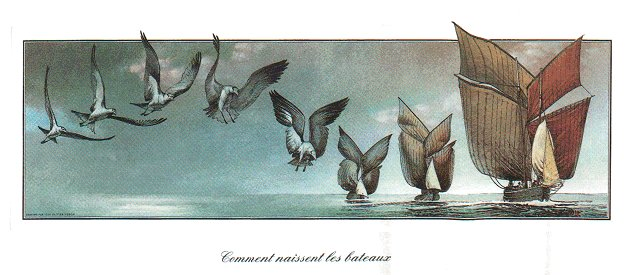
\includegraphics[width=0.9\textheight]{bateaux}}{%
	Caption at top right beside the float and object position right}{fig:9}
\end{lstlisting}

The float can also be put to the left or to the right  (above/below in landscape) with the \texttt{objectPos=l} parameter

\hvFloat[%
	floatPos=p,%
	capWidth=1,%
	capPos=t,%
	rotAngle=90,%
	objectPos=c%
]{figure}{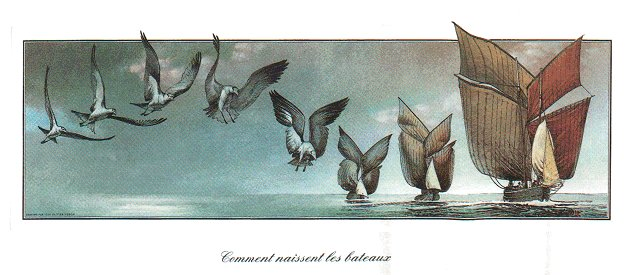
\includegraphics[width=\textheight]{bateaux}}{%
	Caption at top and together with the object rotated}{fig:9}



\hvFloat[%
	floatPos=p,%
	capWidth=h,%
	capPos=r,%
	objectAngle=90,%
	capAngle=-90,%
	objectPos=l%
]{figure}{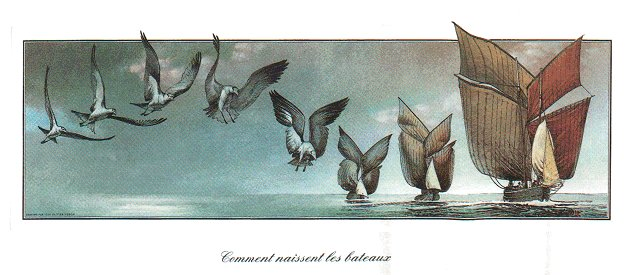
\includegraphics[width=\textheight]{bateaux}}%
	[Rotated Caption]{%
	Caption right beside the float and object position left. The caption rotated by $-90$ degrees}{fig:10}

The code for figure \ref{fig:10}:
\begin{lstlisting}
\hvFloat[%
	floatPos=p,%
	capWidth=h,%
	capPos=r,%
	objectAngle=90,%
	capAngle=-90,%
	objectPos=l%
]{figure}{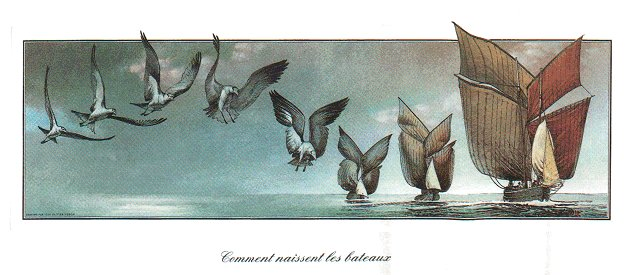
\includegraphics[width=\textheight]{bateaux}}%
	[Rotated Caption]{%
	Caption right beside the float and object position left. The caption rotated by $-90$ degrees}{fig:10}
\end{lstlisting}



\section{The \texttt{nonfloat} Option}
Sometimes it is better to put a "float" in a specific position of the page. This is possible with the \texttt{nonfloat} package and the option \texttt{nonFloat=true}. 

\begin{lstlisting}
\hvFloat[%
	nonFloat=true,%
	capWidth=0.25,%
	capPos=r,%
	capVPos=b,%
	objectPos=c,%
]{figure}{
\includegraphics{rose}}%
	[Nonfloat Captions]{%
	Caption of a "nonfloat" Object, using the \texttt{nonfloat} Package}{fig:11}
\end{lstlisting}

\hvFloat[%
	nonFloat=true,%
	capWidth=0.25,%
	capPos=r,%
	capVPos=b,%
	objectPos=c,%
]{figure}{
\includegraphics{rose}}%
	[Nonfloat Captions]{%
	Caption of a "nonfloat" Object, using the \texttt{nonfloat} Package}{fig:11}

\bigskip
The image \ref{fig:11} is exactly placed where the \texttt{hvFloat} command appears. There are only commands for \texttt{figure} and \texttt{table} environments:

\begin{lstlisting}
\newcommand{\figcaption}{\def\@captype{figure}\caption}
\newcommand{\tabcaption}{\def\@captype{table}\caption}
\end{lstlisting}

But it is no problem, to define more \texttt{xxxcaption} commands to support other with the \texttt{float} package defined new floats.

\section{Tables as Objects}\label{sec:tables}
The object has to be passed as an parameter to the \texttt{hvFloat} macro. This is no problem with images but maybe with tables, so it is easier to use the box \texttt{\textbackslash hvOBox} to save the table in this box and pass it then to \texttt{hvFloat} with the \texttt{useOBox} option. For example see table \ref{table:1} and \ref{table:2}:

\savebox{\hvOBox}{%
\begin{tabular}{l|l|l}
	Name &	Type & Description\\\hline
\texttt{hvFloat}  & command     & places object and caption in different ways\\
\texttt{hvFloatEnv}  & environment & places object and caption exactly Here\\
\texttt{figcaption} & command   & writes a figure caption in a non floating environment\\
\texttt{tabcaption} & command   & writes a table caption in a non floating environment\\
\texttt{setDefaults} & command  & sets all options to the defaults
\end{tabular}
}


\begin{lstlisting}[xrightmargin=-8em,xleftmargin=-3em]
\begin{tabular}{l|l|l}
	Name &	Type & Description\\\hline
	\texttt{hvFloat}  & command     & places object and caption in different ways\\
	\texttt{hvFloatEnv}  & environment & places object and caption exactly Here\\
	\texttt{figcaption} & command   & writes a figure caption in a non floating environment\\
	\texttt{tabcaption} & command   & writes a table caption in a non floating environment\\
	\texttt{setDefaults} & command  & sets all options to the defaults
\end{tabular}
}
\end{lstlisting}

The code for table \ref{table:1} and \ref{table:2} is: 
\begin{lstlisting}[xrightmargin=-7em,xleftmargin=-3em]
\hvFloat[%
	floatPos=!hb,%
	useOBox=true]{table}{}{Demonstration of the \texttt{useOBox} Parameter}{table:1}

\hvFloat[%
	floatPos=hb,%
	useOBox=true,%
	objectAngle=90,%
	capPos=r,%
	capVPos=t,%
	capWidth=0.3]{table}{}{Demonstration of the \texttt{useOBox} Parameter}{table:2}
\end{lstlisting}

In this case leave the third parameter empty.

\hvFloat[%
	floatPos=!hb,%
	useOBox=true]{table}{}{Demonstration of the \texttt{useOBox} Parameter}{table:1}

\hvFloat[%
	floatPos=!htb,%
	useOBox=true,%
	objectAngle=90,%
	capPos=r,%
	capVPos=t,%
	capWidth=0.3]{table}{}{Demonstration of the \texttt{useOBox} Parameter}{table:2}


\section{Text and Objects}\label{sec:text}

With the \texttt{onlyText} option it is no problem to put some text beside an image without getting the caption titels figue/table. The object still can be a floating one or a nonfloating if the \texttt{nonfloat} is used.

\hvFloat[%
	onlyText=true,%
	capAngle=90,%
	capPos=r,%
	capVPos=t,%
	capWidth=h]{}{
\includegraphics{rose}}%
	["\texttt{onlyText}" Caption]{%
	Demonstration of the \texttt{onlyText} Parameter, which makes it 
	possible to put some text beside a floating object without getting 
	a starting \texttt{Figure:} or \texttt{Table:}}{fig:text}

The code for figure \ref{fig:text}:


\begin{lstlisting}
\hvFloat[%
	onlyText=true,%
	capAngle=90,%
	capPos=r,%
	capVPos=t,%
	capWidth=h]{}{
\includegraphics{rose}}%
	["\texttt{onlyText}" Caption]{%
	Demonstration of the \texttt{onlyText} Parameter, which makes it 
	possible to put some text beside a floating object without getting 
	a starting \texttt{Figure:} or \texttt{Table:}}{fig:text}
\end{lstlisting}



\section{Environment \texttt{hvFloatEnv}}\label{sec:env}

With the environment \texttt{hvFloat} one can place an object exactly on that position where the
environment is defined. For captions the use of \CMD{captionof} is recommended:

\begin{hvFloatEnv}
\captionof{table}{A caption for a nice table}
\begin{tabular}{@{} l c r @{}}\hline
left & center & right \\
L    & C      & R     \\\hline
\end{tabular}
\end{hvFloatEnv}

\begin{lstlisting}
\begin{hvFloatEnv}
\captionof{table}{A caption for a nice table}
\begin{tabular}{@{} l c r @{}}\hline
left & center & right \\
L    & C      & R     \\\hline
\end{tabular}
\end{hvFloatEnv}
\end{lstlisting}

The environment has an optional argument for setting the line width which is preset to \CMD{textwidth}.
The object is always centered.

\begin{hvFloatEnv}[0.5\textwidth]
\captionof{table}{A caption for a nice table}
\begin{tabular}{@{} l c r @{}}\hline
left & center & right \\
L    & C      & R     \\\hline
\end{tabular}
\end{hvFloatEnv}

\begin{lstlisting}
\begin{hvFloatEnv}[0.5\textwidth]
\captionof{table}{A caption for a nice table}
\begin{tabular}{@{} l c r @{}}\hline
left & center & right \\
L    & C      & R     \\\hline
\end{tabular}
\end{hvFloatEnv}
\end{lstlisting}


%\appendix
%\section{Problems}
%\begin{itemize}
%\item[] With the \texttt{nonfloat} option all objects are left aligned, \verb|\centering| doesn't work here. Only God knows why ...\hfill \textbf{solved!}
%\end{itemize}



\section{The Package Source}
\lstinputlisting[basicstyle=\ttfamily\footnotesize,tabsize=3]{hvfloat.sty}


\end{document} 

